\section{Experiments}
\subsection{Counterexample: the mechanism is visible}
We reproduce the source recurrence using its random-time law $\mathbb P(r\le b)=\sqrt b$, independent child trees in each multilevel difference, and matched random trees across methods. We test $d\in\{2,5,10,20,50,100,200,500,1000\}$ and $n=m\in\{1,2,3,4\}$ with 512 estimator replicas per configuration. Time and active-coordinate streams are coupled across dimensions, so a flat subspace-IR curve is an expected consequence of the theorem rather than post-hoc smoothing. We separately validate the closed-form MSE with 65,536 fresh Gaussian replicas for each $N\in\{1,4,27,256\}$.

\begin{table}[t]
\caption{Full-state RMSE at $n=m=3$ ($N=27$).}
\label{tab:counter}
\centering\small
\begin{tabular}{rrrrr}
\toprule
$d$ & Raw MLP & Final only & Unit ball & Subspace IR\\
\midrule
2&1.196&0.939&0.776&0.356\\
10&12.767&5.412&1.358&0.356\\
100&504.759&66.088&1.427&0.356\\
1000&16995.683&697.972&1.434&0.356\\
\bottomrule
\end{tabular}
\end{table}

\begin{figure}[t]
\centering
\IfFileExists{figures/counterexample_state_rmse.pdf}{\includegraphics[width=\columnwidth]{figures/counterexample_state_rmse.pdf}}{\fbox{\parbox[c][26mm][c]{.92\columnwidth}{\centering Figure asset is included in the Overleaf package.}}}
\caption{The unprojected full-state error worsens with ambient dimension; recursively enforcing the certified subspace is flat and matches reduced Monte Carlo.}
\label{fig:counter}
\end{figure}

At $d=1000$, raw MLP and final-only projection have the same value RMSE, $396.978$, whereas recursive subspace IR has value RMSE $0.119$. Thus the gain is not an artifact of deleting gradient coordinates from the final metric. The exact RMSE prediction in~\eqref{eq:exactmse} matches an independent Gaussian-moment validation to within $0.56\%$ across $N\in\{1,4,27,256\}$.

\subsection{Broader benchmarks}
We next ask whether the same mechanism appears when the restricted generator is not identically zero or when the certificate is a ball/ellipsoid rather than a subspace. Certificates are derived independently of realized numerical error; details are in Appendix~\ref{app:certificates}.

\paragraph{Quadratic HJB.}
For the Rosenbrock benchmark, the non-oracle ball $\norm z\le\sqrt{15}$ reduces mean relative $L_2$ error from $2.08$--$2.49$ to $0.63$--$0.64$ across $d=100$--$160$. To test the mechanism rather than only final error, we evaluate the same intermediate states against a stable Hopf--Cole reference. Generator MSE falls by $98.9$--$99.6\%$, and the variance across paired runs of the actual first nonlinear level correction falls by $98.8$--$99.7\%$. These diagnostics directly measure the two quantities the proposed mechanism predicts should shrink.

\begin{figure*}[t]
\centering
\begin{minipage}{0.48\textwidth}
\centering\IfFileExists{figures/hjb_generator_mse.pdf}{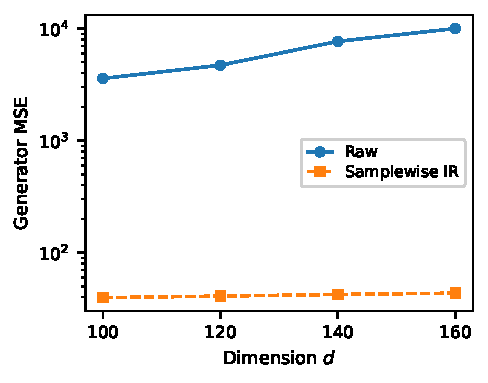
\includegraphics[width=\linewidth]{figures/hjb_generator_mse.pdf}}{\fbox{\parbox[c][22mm][c]{.92\linewidth}{\centering Figure asset is included in the Overleaf package.}}}\\[-1mm]
{\small (a) Generator MSE}
\end{minipage}
\hfill
\begin{minipage}{0.48\textwidth}
\centering\IfFileExists{figures/hjb_correction_variance.pdf}{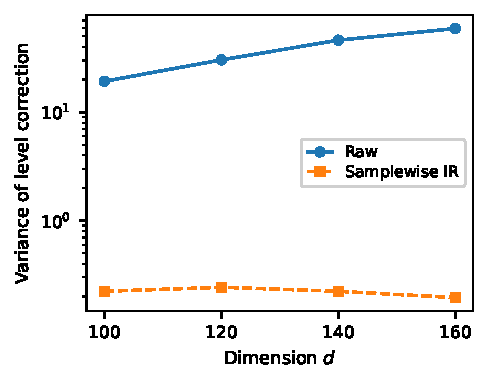
\includegraphics[width=\linewidth]{figures/hjb_correction_variance.pdf}}{\fbox{\parbox[c][22mm][c]{.92\linewidth}{\centering Figure asset is included in the Overleaf package.}}}\\[-1mm]
{\small (b) Nonlinear level-correction variance}
\end{minipage}
\caption{Mechanism diagnostics for the high-dimensional HJB benchmark. The certified projection suppresses both nonlinear generator error and the variance of the actual recursive correction.}
\label{fig:hjbdiag}
\end{figure*}

\paragraph{Neufeld--Wu.}
In the published 100--300D gradient-dependent example, a model-derived gradient envelope lies far below the threshold where the driver activates. At small budgets, Samplewise IR reduces MAE by $47.5$--$71.4\%$ over 30 runs.

\paragraph{100D nonlinear funding.}
A state-dependent ellipsoid in normalized delta coordinates reduces MAE from $1.336$ to $0.495$ at one representative budget ($n=2,M=10$), and from $1.100$ to $0.394$ at a larger one ($n=3,M=8$).

\begin{table}[t]
\caption{Paired Samplewise IR vs. Batch-IR. Lower is better.}
\label{tab:batch}
\centering\small
\begin{tabular}{llrrr}
\toprule
problem & setting & raw & sample & batch\\
\midrule
HJB & $d=20,M=6$ &314.136&0.2412&\textbf{0.0966}\\
HJB & $d=40,M=6$ &1034.262&0.1993&\textbf{0.0833}\\
Funding & $M=10$ &1.4042&0.5102&\textbf{0.4807}\\
Funding & $M=20$ &0.8848&0.2965&\textbf{0.2539}\\
Funding & $M=40$ &0.5221&0.1993&\textbf{0.1486}\\
\bottomrule
\end{tabular}
\end{table}

\paragraph{Samplewise vs. batchwise.}
Table~\ref{tab:batch} shows that a common feasible scale can outperform nearest-point projection in low-budget HJB and funding tests. A mean-preserving contraction is also useful once the raw batch mean is feasible, showing that variance suppression can help even without moving the mean. On the thresholded Neufeld--Wu driver, Samplewise IR and Batch-IR are numerically identical: either correction prevents the same spurious activation. We therefore view the methods as complementary, not ordered.

\paragraph{Negative controls.}
Projection leaves value error unchanged in a linear convection--diffusion problem where $z$ is not reused nonlinearly. It is also numerically inert in a 100D credit-risk test where the certified interval is almost never violated, and in 100D Allen--Cahn at the tested budget where the maximum-principle interval is never left. These controls argue against a generic ``clipping helps'' explanation.

\section{What the Experiments Establish}
The counterexample separates a structural claim from a statistical design choice. The structural claim is that recursive infeasibility can create a spurious nonlinear source, and that a generator-compatible certificate can remove it exactly. The statistical choice is how to move noisy samples into the feasible set. Equation~\eqref{eq:pyth} favors nearest-point projection for one-state Euclidean error; Table~\ref{tab:batch} shows that a common batch scale can nevertheless be better after nonlinear recursion. This is not a contradiction: two complete recursive schemes generate different later states, and the batch method deliberately trades bias for stronger spread suppression.

A mean-preserving batch diagnostic sharpens the point. When the raw batch mean is feasible, shrinking deviations around that mean can improve final error without changing the empirical mean. When the batch mean itself is outside a convex feasible set, no all-feasible mean-preserving correction exists, because the mean of feasible points must be feasible. Thus low-budget high-dimensional failure can affect the batch center as well as isolated outliers.

\section{Related Work and Limitations}
MLP theory establishes high-dimensional convergence and polynomial complexity for several semilinear PDE classes, including gradient-dependent nonlinearities \citep{E2021,HutzenthalerKruse2020,NeufeldWu2025,NeufeldNguyenWu2025}. Truncated MLP has been used for locally Lipschitz Allen--Cahn reactions \citep{Beck2020}. Our point is different: use PDE-certified geometry of the value--gradient state before nonlinear recursive reuse. Hard-constrained neural networks enforce constraints by construction in learned predictors \citep{Min2024}; here the constraint acts inside a stochastic numerical recursion. SCaSML uses learned PDE surrogates with MLP defect correction \citep{Fan2026}; our mechanism is orthogonal and can modify the stochastic correction engine itself.

The exact rescue assumes known certified structure rather than discovering it. Approximate or learned subspaces require misspecification analysis. Samplewise consistency inherits the regularity, moment, and measurability assumptions of existing MLP theory. Batch-IR changes dependence and finite-sample bias; we deliberately leave its sharp consistency and complexity theory to future work. Finally, a misspecified feasible set can bias the target, so certificates must come from PDE/model structure rather than test-error tuning.

